%forklar toolchain skidtet
%regneark med data - parameter til python - til cora model - til cora verifyta - til læsbart trace - til python - til SMC model - til query - til python - til start/til scheule
\section{Tool-chain} \label{sec:tool_chain}
\afx{Før dette læses, så er de diverse tools blevet introduceret. Her er CSV fil formattet også forklaret}\\
In order to clarify our usage of different tools we will in this section describe the different steps in our system. \Cref{fig:tool_chain} displays the flowchart representation of the tool-chain. The numbers that are used are only there for the convenience of this section as we will present some of the locations, some will be excluded as they are trivial or similar to another location. 

\paragraph{Location 1 - CSV file that contains payload information} is the input file for the system. The usage of this file and its format is described in \cref{sec:csvlang}.

\paragraph{Location 2 - Generate \gls{cora} XML models file from input} in this location we will read the CSV file or the tuned parameters from location 9. The input is used to generate two \gls{cora} models. One model uses the worst case values and the other will use the values from the CSV file. 

%\paragraph{Location 3 - Input model to CORA Verifyta} the Verfyta will generate a trace for each model.

\paragraph{Location 4 - Test worst case model} run the queries on the worst case model.

\paragraph{Location 5 - Is the worst case possible?} If we were unable to produce a trace for the worst case, we will not be able to guarantee that any of the schedules we produce will stay within the specified parameters. We will as a result thereof go to location 6, the fail state.

\paragraph{Location 7 - Extract trace from the \gls{cora} model and it to LIBUTAP}
In this location we will extract a trace from the \gls{cora} model and use it as input for the tracer function in LIBUTAP. The tracer function will transform the output into a readable trace which can be used later on.

%\paragraph{Location 9 - Convert trace to \gls{smc} xm model file} in this location we will read the trace and produce the \gls{smc} model that will be used in the next location.

\paragraph{Location 10 - Verify queries and extract the results} the \gls{smc} Verifyta will run the queries on the \gls{smc} model and output the results, see \cref{sec:smc}. These queries is made to validate and test the robustness of the trace.

\paragraph{Location 13 - Output schedule} if the queries are satisfied we will output the schedule, as this will indicate that the trace, or schedule, is correct.

\paragraph{Location 12 - Tune model parameters} if the queries were not satisfied, the schedule will be discarded and we will produce a new one. In order to produce a new schedule, we will provide \gls{cora} with a new set of parameters based on those from the CSV file. These parameters will be loyal to those specified in the CSV file, but their ranges will be shortened in order to provoke new choices in the schedule. This will change the workflow as we are not interested in verifying the worst case model any more, as the previous worst case is still true to this version of the parameters. We will therefore skip location 4, 5, and 6 and will go directly yo location 7.

\begin{figure}
	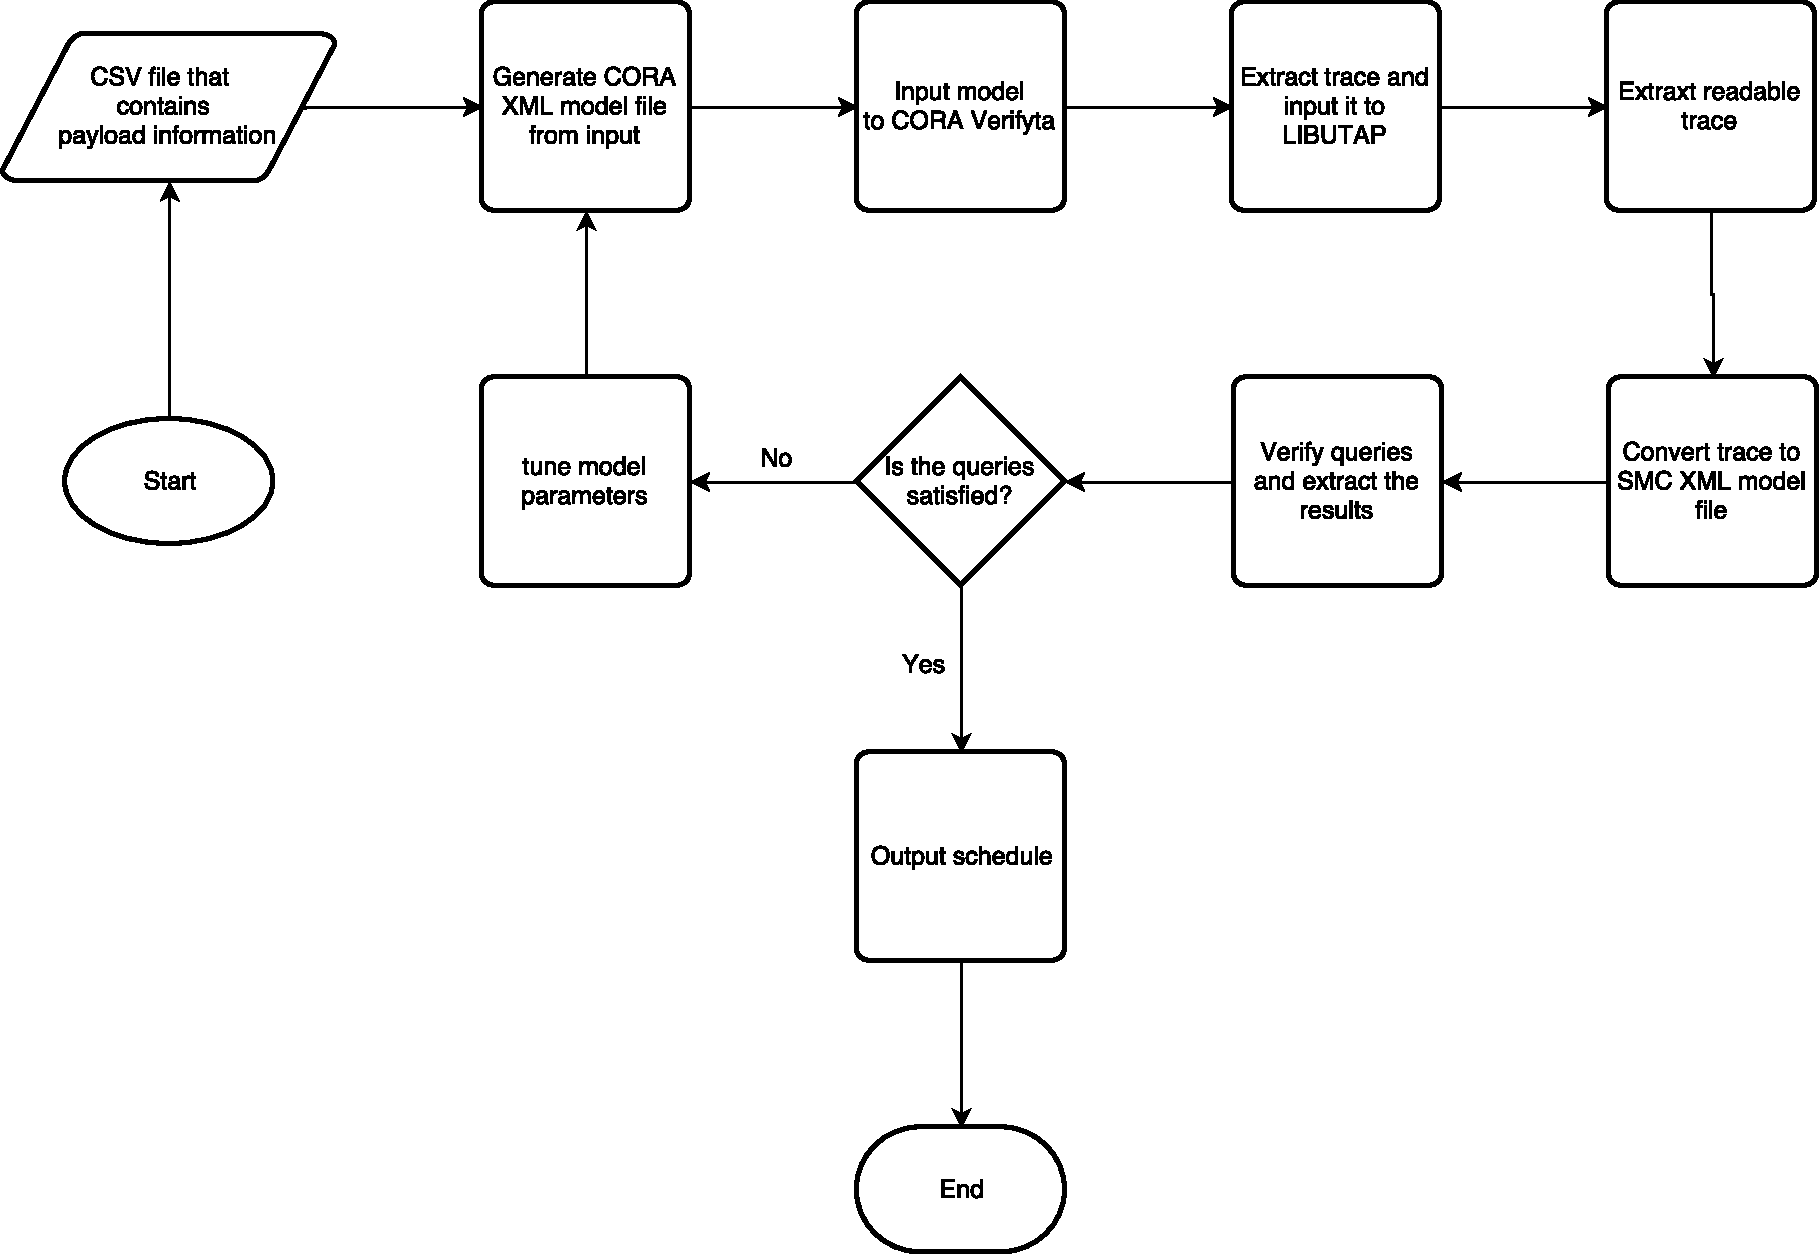
\includegraphics[width=\textwidth]{graphics/tool_chain.pdf}
	\label{fig:tool_chain}
	\caption{Flowchart that displays the worflow and use of tools}
\end{figure}
